\section{Theoritical background}\label{Theory}
\subsection{Side-channel attack}
\textit{Side-Channel Attack} (SCA) refers to attacks that take advantage 
of any form of leakage of a device to find information about its sensitive 
variables (i.e. its cryptographic key). Introduced by \textit{Kocher et 
al} in \cite{KocherDPA}, they are nowadays used to evaluate the resilience 
of processors against physical attacks. Those attacks can be invasive, by 
disrupting the behavior of the device, or they can just monitor the 
behavior and not interfere with the device operations. \\

The non invasive attacks are called as \textit{Side-Channel Analysis 
Attacks} (SCAA) because they only analyze the device behavior. They 
exploit the information carried by the leakage and compare it with the 
knowledge of the plaintexts encrypted. Their exists many types of SCAA, 
depending on the type of leakage used. It gives different SCAA such as 
timing, electromagnetic or power analysis attacks. Timing attacks 
\cite{KocherTiming,} exploit non constant time execution of an algorithm 
due to branches, cache misses, etc. Electromagnetic attacks 
\cite{electromagnetic} use the electromagnetic radiations emitted whereas 
\textit{Power Analysis Attack} (PAA) takes advantage of the power 
consumption of the device during the encryption.\\

One of the most important PAA is the \textit{Differential Power Analysis} 
(DPA). Firstly presented in \cite{KocherDPA}, DPA works on the principle 
that the power consumption is related to the values being manipulated. 
Therefore recording the power consumption during the encryption should 
give information about the key used. It is based on divide-and-conquer 
principle where, instead of recovering the full key at once, each byte of 
the key is attacked independently. This helps to reduce the complexity of 
the attack as well as its time execution. \\

The DPA is usually performed in two phases:

First, a training phase can be conducted by the attacker where he collects 
multiple traces for different known plaintexts and keys. The goal of the 
training phase is to profile and model the leakage of a device when it 
manipulates a sensitive variable.  To do so, the attacker chooses a model 
following the leakage and characterize it thanks to the training traces. 
For instance, one could assume that the each sample of the leakage follows 
a gaussian distribution and the training traces are used to compute the 
corresponding mean and standard deviation. In the end, the training phase 
aims to obtain a model for every internal state value. 

Second, the attacker tries to recover the value of the sensitive variables 
for new leakages. To achieve this, he uses the trained model on the new 
traces to derive different probabilities associated to the sensitive 
variable value. The highest probability should correspond to the correct 
internal state value if the model corresponds to the actual leakage 
distribution.\\

In this thesis, one will focus on recovering the 128 bits key used during 
an AES encryption by using a divide and conquer DPA called template 
attack.
\subsection{AES}\label{sect:AES}
The \textit{Advanced Encryption Standard} (AES), also known as Rijnadel, 
is a block cipher based on a substitution-permutation network developed by 
Joan Daemen and Vincent Rijmen and whose specifications are described in 
\cite{AES_spec}. It is a symmetric encryption algorithm (encryption and 
decryption use the same key) which operates with key sizes of 128, 192 or 
256 bits. The block diagram of the AES execution can be seen in Figure 
\ref{fig:aes building block}. 
\begin{figure}[h]
    \centering
    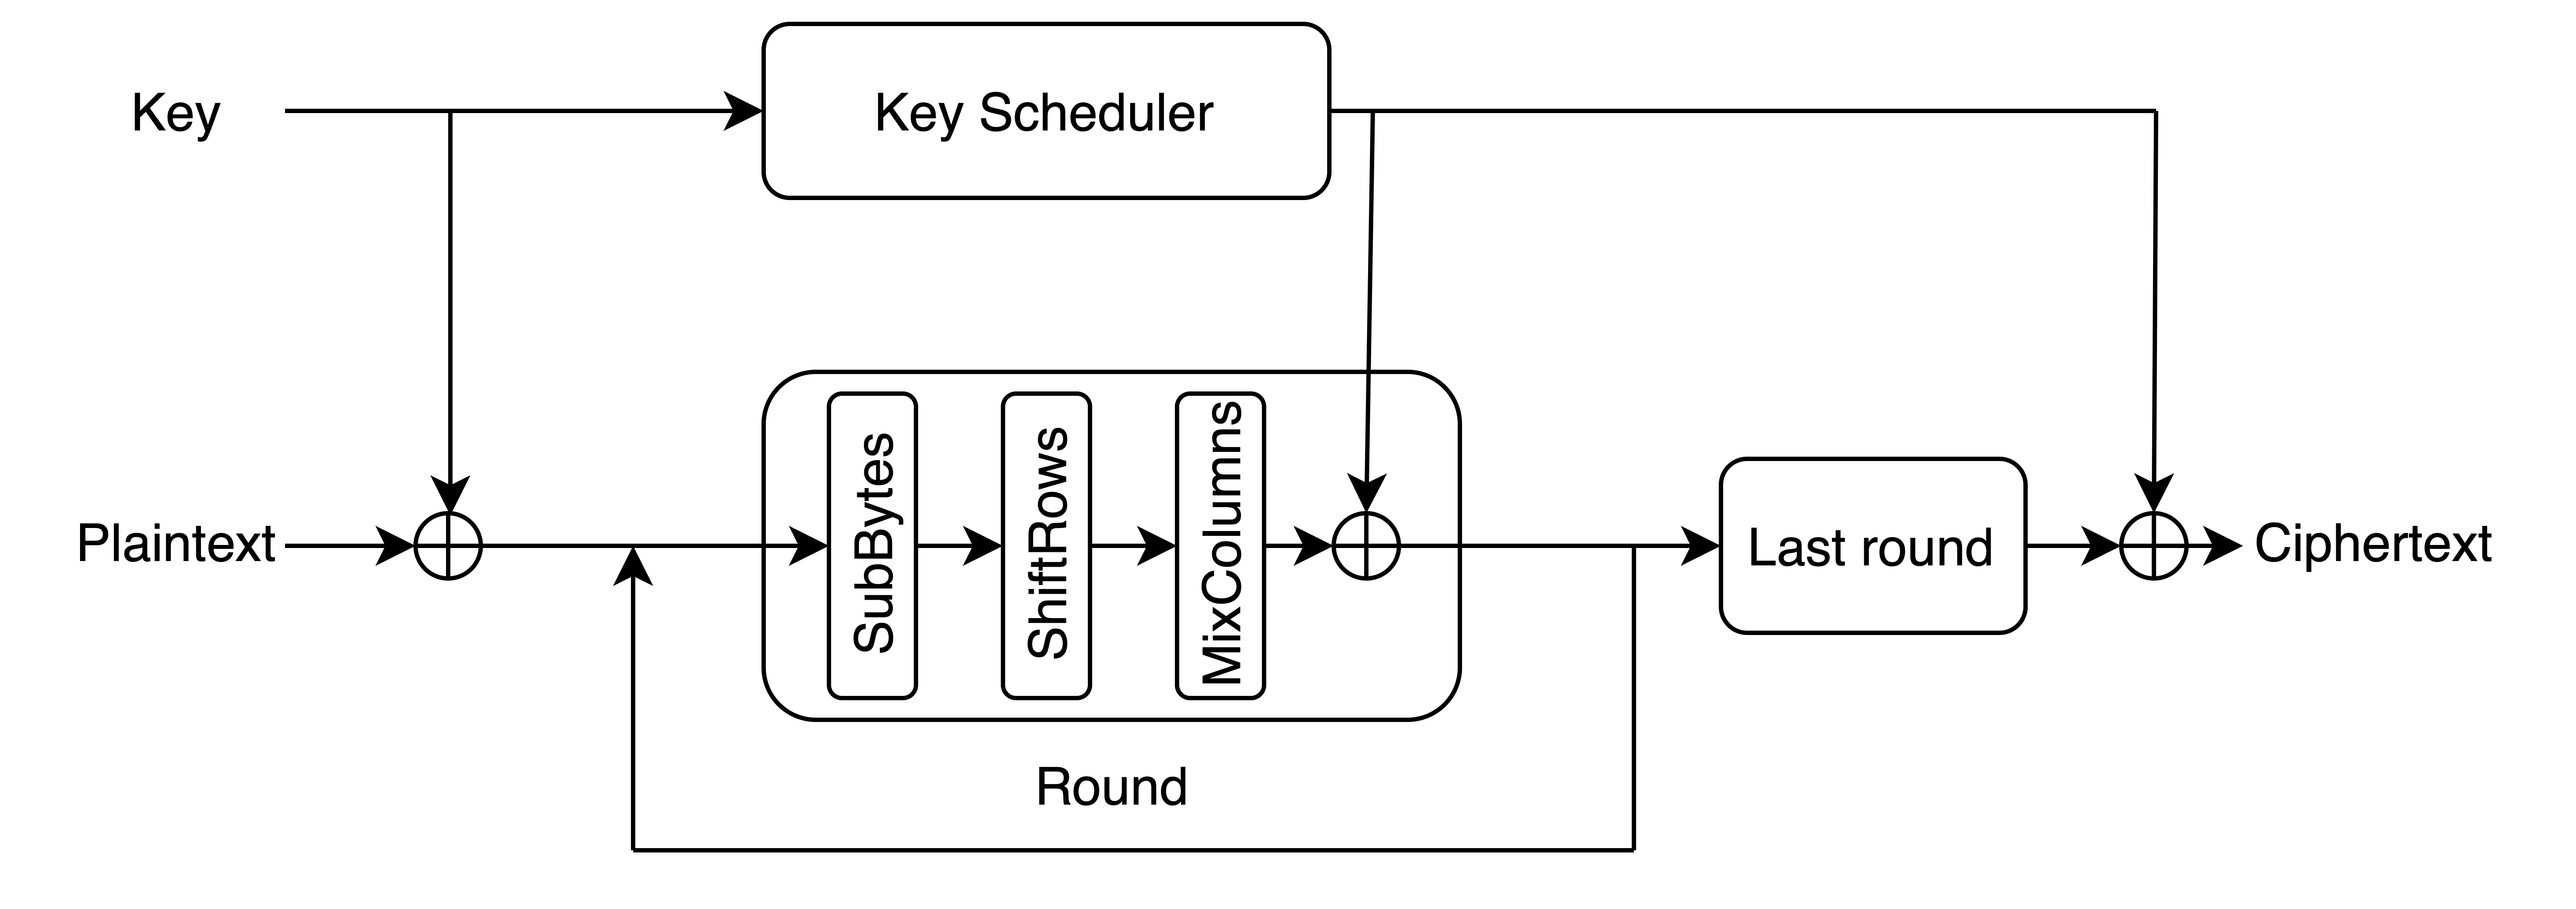
\includegraphics[scale=0.7]{Images/AES schematic.png}
    \caption{Block diagram of the AES encryption}
    \label{fig:aes building block}
\end{figure}
As illustrated, the AES performs the same operations multiple times, this 
operation, called round, is performed $n$ times where $n$ depends on the 
key size. For key size of 128, 192 or 256 bits, it is executed 
respectively 10, 12 or 14 rounds. The operations executed within a round 
are denoted the building blocks and are described in the following. A 
different key is used for each round and those different 128 bits keys are 
derived from the initial one thanks to a key expansion algorithm. One 
should notice that the key used for the first round corresponds to the 
initial key and the DPA against AES are therefore focusing the first round 
of the execution. This is the reason why the key expansion algorithm will 
not be described in the following. Moreover, only 128 bits key size will 
be investigated in this work and for now on, AES will refer to AES with 
128 bits key size.


\subsubsection{Buidling blocks}
The AES operates on $4\times4$ matrix of bytes to represent the different 
internal states during the encryption. Let $\mathbf{s}^r$ be the state 
matrix at the beginning of the round $r$ where the initial state 
$\mathbf{s}^0$ stores the 16 bytes of the 128 bits plaintext. The 
encryption is performed by different blocks working with arithmetic in 
$\mathbb{F}_{2^8}$.
\begin{equation*}
    \mathbf{s}^r = \begin{bmatrix}
B_0^r & B_4^r & B_8^r    & B_{12}^r\\
B_1^r & B_5^r & B_9^r    & B_{13}^r\\
B_2^r & B_6^r & B_{10}^r & B_{14}^r\\
B_3^r & B_7^r & B_{11}^r & B_{15}^r
\end{bmatrix}
\end{equation*}
\textbf{AddRoundKey} : The Add Round Key ensures key mixing thanks to a 
bitwise XOR between the state and the key. This is used to have a keyed 
permutation such as only the receiver, knowing the key, can decrypt the 
ciphertext.
\begin{equation*}
    \text{AddRoundKey}(\mathbf{s}^r) = \mathbf{s}^r \oplus \mathbf{k}^r = 
\begin{bmatrix}
B_0^r\oplus K_0^r & B_4^r\oplus K_4^r & B_8^r   \oplus K_{8}^r  & 
B_{12}^r\oplus K_{12}^r\\
B_1^r\oplus K_1^r & B_5^r\oplus K_5^r & B_9^r   \oplus K_{9}^r  & 
B_{13}^r\oplus K_{13}^r\\
B_2^r\oplus K_2^r & B_6^r\oplus K_6^r & B_{10}^r\oplus K_{10}^r & 
B_{14}^r\oplus K_{14}^r\\
B_3^r\oplus K_3^r & B_7^r\oplus K_7^r & B_{11}^r\oplus K_{11}^r & 
B_{15}^r\oplus K_{15}^r
\end{bmatrix}
\end{equation*}
\textbf{SubBytes} SubBytes is the operation responsible of the confusion. 
It performs an inversion in $\mathbb{F}_{2^8}$ followed by an affine 
transformation on each byte. 
\begin{equation*}
     \text{SubBytes}(B^r_i) = \text{affine}\Bigl((B_i^r)^{-1}\Bigr)
\end{equation*}
\begin{equation*}
    \text{affine}(B) = \begin{bmatrix}
     1 & 0 & 0 & 0 & 1 & 1 & 1 & 1\\
     1 & 1 & 0 & 0 & 0 & 1 & 1 & 1\\
     1 & 1 & 1 & 0 & 0 & 0 & 1 & 1\\
     1 & 1 & 1 & 1 & 0 & 0 & 0 & 1\\
     1 & 1 & 1 & 1 & 1 & 0 & 0 & 0\\
     0 & 1 & 1 & 1 & 1 & 1 & 0 & 0\\ 
     0 & 0 & 1 & 1 & 1 & 1 & 1 & 0\\
     0 & 0 & 0 & 1 & 1 & 1 & 1 & 1
    \end{bmatrix}
    \begin{bmatrix}
        b_0 \\ b_1 \\ b_2 \\ b_3 \\ b_4 \\ b_5 \\ b_6 \\ b_7
    \end{bmatrix} + 
    \begin{bmatrix}
        1 \\ 1\\ 0 \\ 0 \\ 0 \\ 1 \\ 1 \\ 0
    \end{bmatrix}
\end{equation*}
In the affine transformation, $b_0$ and $b_7$ corresponds respectively to 
the MSB and LSB of the byte $B$. SubByte is the only non-linear block of 
the AES and can be precomputed to create a \textit{substitution box} or 
S-Box, a table of $256$ elements containing the corresponding output.\\

\textbf{ShiftRows} : ShiftRows is one of the block performing the 
diffusion. It performs a circular left shift on each row with a shift 
value depending on the row index (left shift of $i$ for the row $i$). In 
hardware, this can be implemented by a simple wire crossing.
\begin{equation*}
    \text{ShiftRows}(\mathbf{s}^r) = \begin{bmatrix}
B_0^r    & B_4^r    & B_8^r    & B_{12}^r\\
B_5^r    & B_9^r    & B_{13}^r & B_1^r\\
B_{10}^r & B_{14}^r & B_2^r    & B_6^r\\
B_{15}^r & B_3^r    & B_7^r    & B_{11}^r
\end{bmatrix}
\end{equation*}
\textbf{MixColumns} : MixColumns is the second block performing diffusion. 
Each column is associated to a polynomial such that $a(x)= a_3 x^3 + a_2 
x^2 + a_1 x + a_0$ where $a_i$ is the $i^\text{th}$ byte, of the column. 
This polynomial is then multiplied by another fixed one 
$c(x)=03x^3+02x^2+01x+02$ $\text{mod}$ $x^4+1$. This can be written as a 
matrix multiplication where $\mathbf{s}^r_{i,j}$ denotes the $j^\text{th}$ 
byte of the $i^\text{th}$ column of $\mathbf{s}^r$.
\begin{equation*}
    \text{MixColumns}(\mathbf{s}^r_i) = \begin{bmatrix}
        02 & 03 & 01 & 01 \\
        01 & 02 & 03 & 01 \\
        01 & 01 & 02 & 03 \\
        03 & 01 & 01 & 02
    \end{bmatrix}
    \begin{bmatrix}
        \mathbf{s}^r_{i,0}\\
        \mathbf{s}^r_{i,1}\\
        \mathbf{s}^r_{i,2}\\
        \mathbf{s}^r_{i,3}
    \end{bmatrix}
\end{equation*}
\subsection{Divide and Conquer approach}
The AES uses a 128 bits key size. One could attack this 128 bits key at 
once by enumerating all the $2^{128}$ different possible values. Even if 
this attack is theoretically possible, in practice exhaustive key search 
is too long to be successful. To reduce the number of possible values in 
the enumeration process, one could try to attack more keys of smaller 
sizes called \textit{sub-keys}. For instance, attacking 4 sub-keys of 32 
bits or 32 sub-keys of 4 bits. This approach is called a \textit{divide 
and conquer} attack. \\

The AES is originally designed not to encrypt the 128 bits plaintext at 
once but by encrypting it using arithmetic in in $\mathbb{F}_{2^8}$. It 
implies that the 128 bits are sometimes manipulated by block of 8 bits and 
this operation is repeated 16 times. This behavior can be seen during the 
AES encryption with the SubBytes block which operates the inverse 
operation in $\mathbb{F}_{2^8}$ on the 16 bytes independently. Moreover, 
this block is also the only non-linear block of the AES execution. It 
means that two similar plaintexts (i.e. differing from one bit) encrypted 
with the same key can have  more than one bit of difference at the output 
of SubBytes. This would not have been the case with a linear block such as 
xoring .\\

SCA commonly focuses on the output of the SubByte operation of the first 
round. This place is chosen because of the non-linear behavior of the 
SubByte block but also because the secret key is xored with the plaintext 
just before this block. As those operations does not affect more than 8 
bits together it is a good place to operate a divide and conquer attack 
where each attack targets the output of one S-Box. Finally, there are 16 
independent attacks on 8 bits.
\textcolor{red}{Add figure}
\subsection{Training phase}\label{sec:Training phase}
In the training phase, the attacker is able to record the leakage of many 
encryptions with different plaintexts and keys that are both known. This 
set of leakage and its corresponding data is referred to as the 
\textit{training set}. The goal of the training phase is to use the 
training set in order to profile the leakage of the device. This leakage 
follows a certain distribution that is unknown by the attacker and which 
depends on the value of the internal state (i.e. the ouptut of the S-Box). 
A statistical model must be selected to represent the unknown leakage 
distribution for a given internal state value and the training set is then 
used to estimate the model's parameters. At the end of the training phase, 
16 attacks are built where each of them is focusing on the S-Box output. 
One will only present how to construct the attack for one S-Box, the 
combination of the 16 S-Boxes will be shown in section \ref{sec:Attack 
phase}.\\

One attack is composed of 256 models, one for each 8 bits S-Box output 
value. In this section, one will firstly present how to choose and build 
the model from the training set. Then, one will introduce some tools, 
relying on information theory, that measures the quality of the model 
built.

\subsubsection{Point of Interest}
The recorded leakage traces contain samples that can be relevant or 
irrelevant depending on which internal state is modeled. For instance, 
Figure \ref{fig:trace recorded} shows the execution of AES encryption. The 
attack focuses on the first round of the encryption thus the samples 
associated to the other rounds could be not useful. The relevant samples 
are commonly called \textit{Point of Interest} (POI). They should be well 
chosen in order to fit accurately the model to the true leakage 
distribution of the device. Moreover, even if all samples of the first 
round can be useful, some of them could give more information than others. 
For instance, the samples acquired at the same time as the processor 
loaded the S-Box output are much more informative than others samples. 
There exists a statistical tool for finding those most informative POI 
which is called \textit{Signal-to-Noise Ratio} (SNR).
\begin{figure}[h]
    \centering
    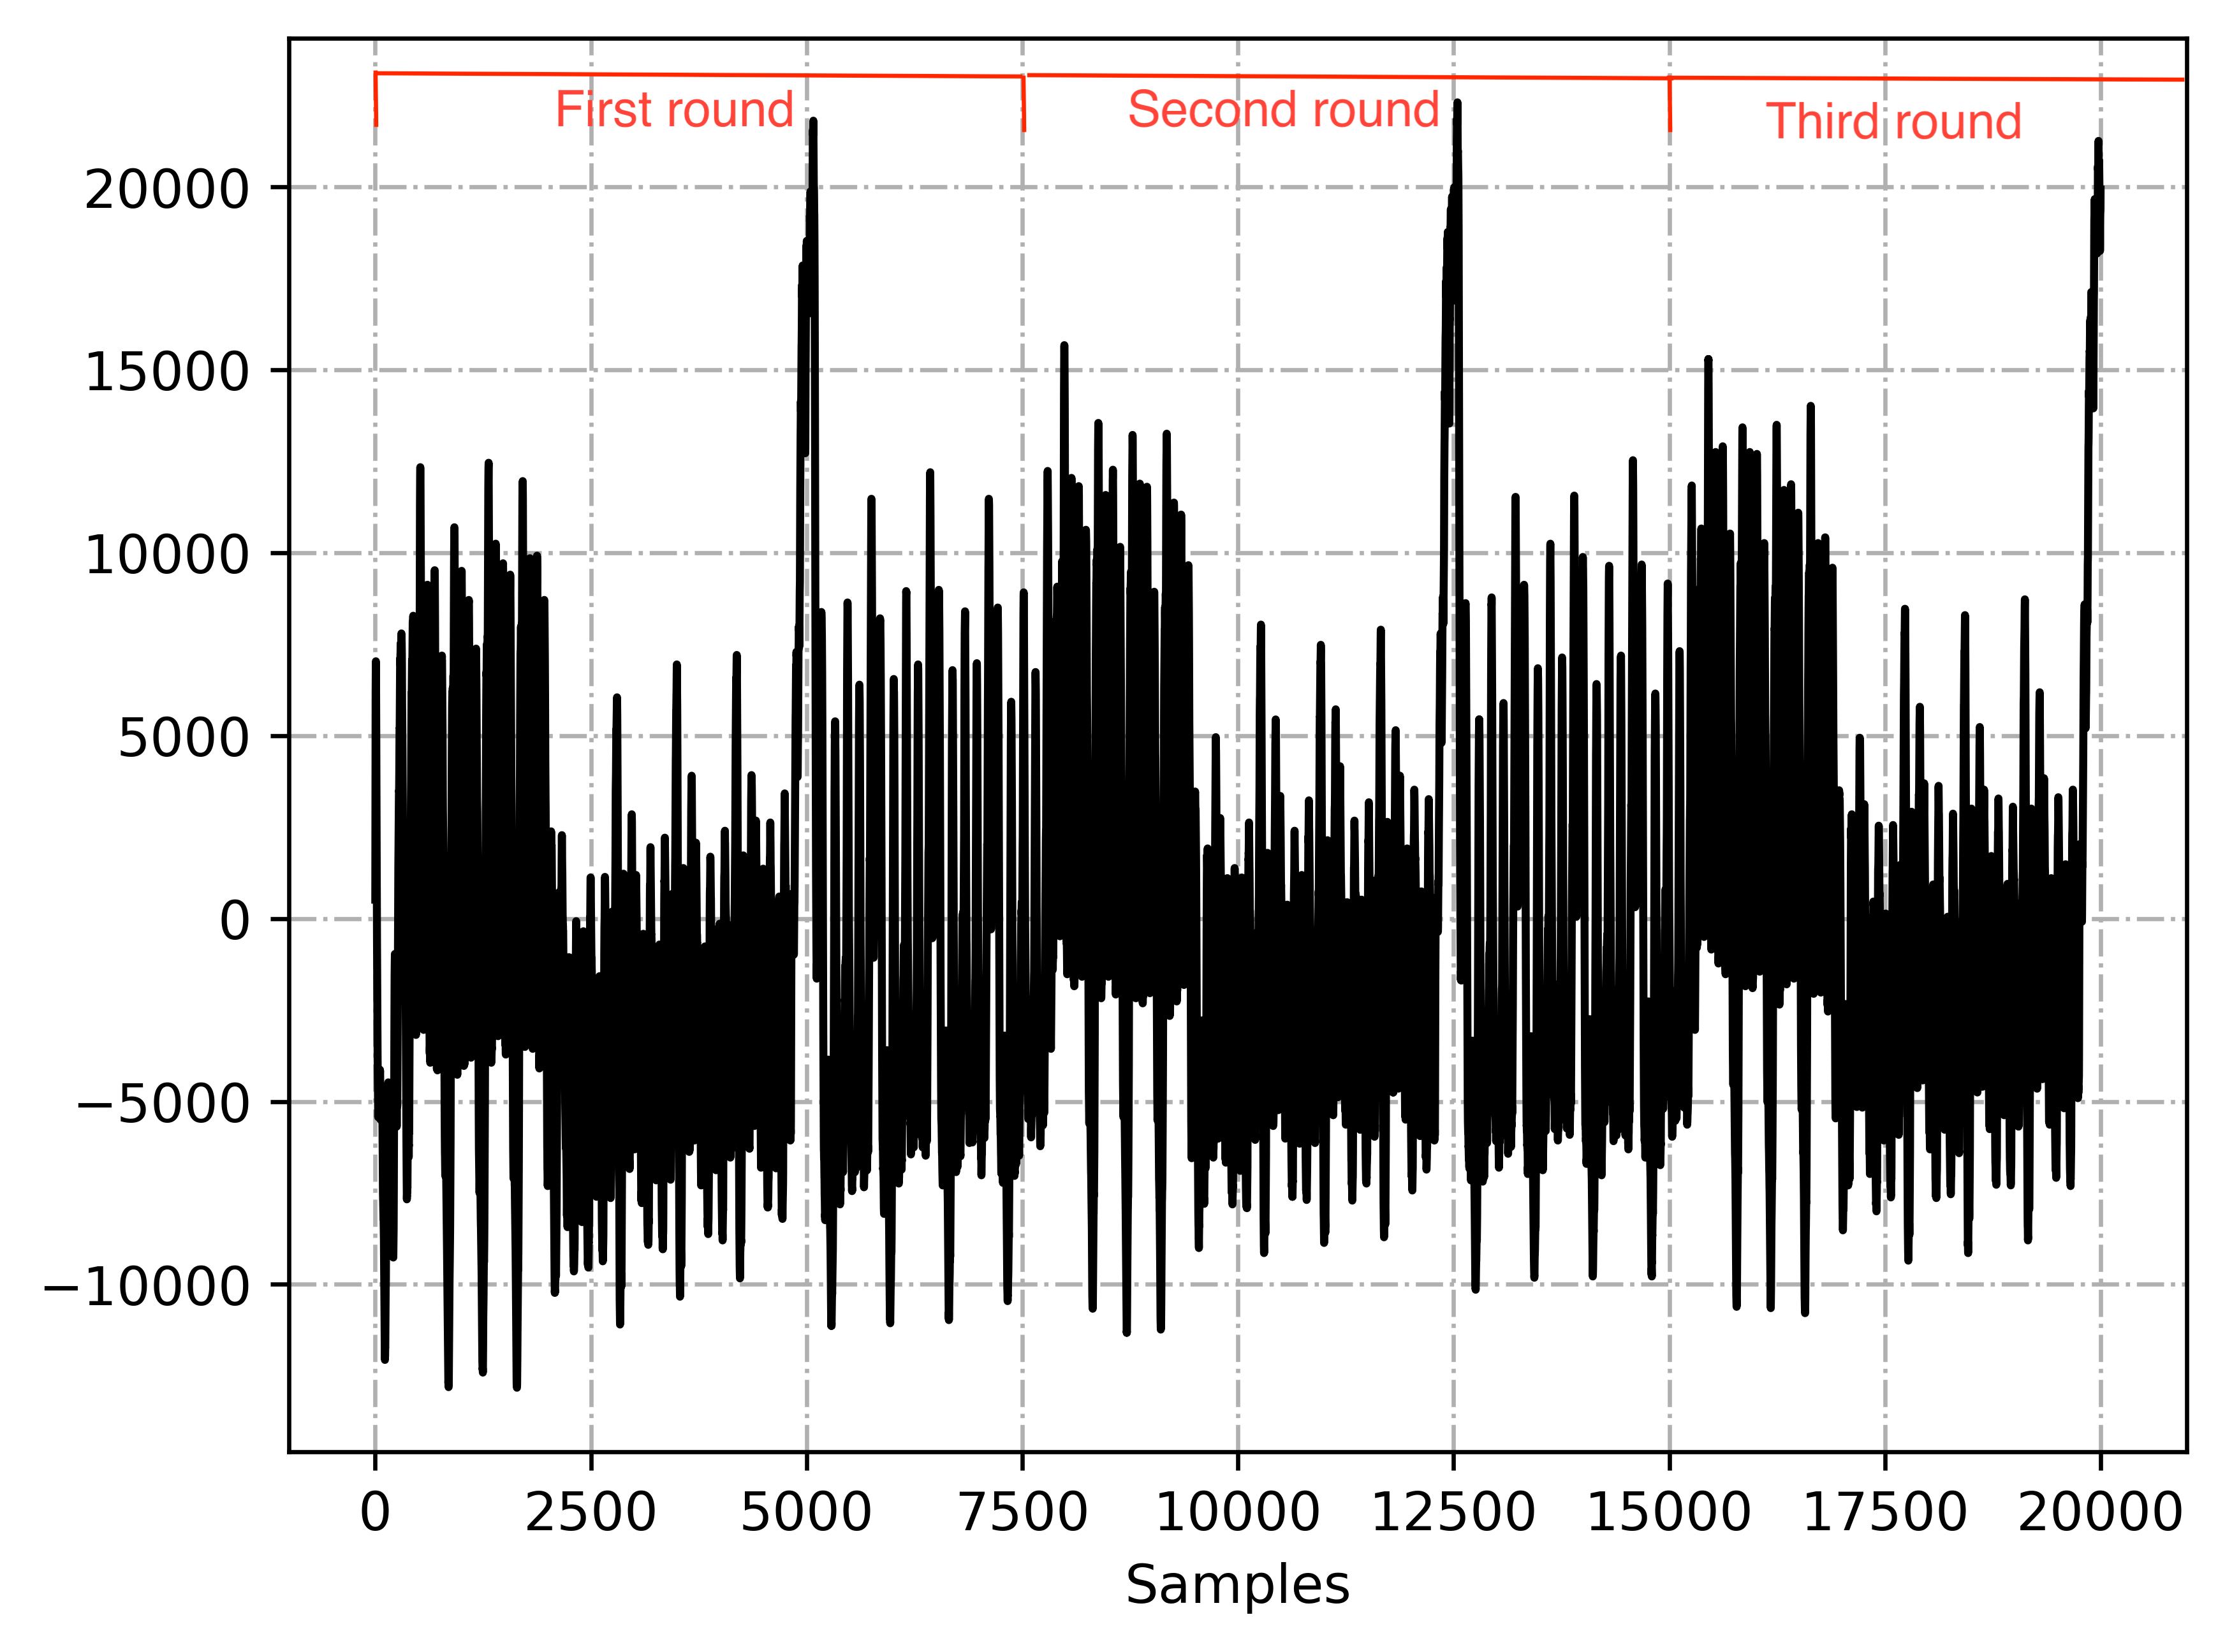
\includegraphics[width=0.5\columnwidth]{Images/Trace recording.png}
    \caption{First three round of an AES encryption}
    \label{fig:trace recorded}
\end{figure}
\subsubsection{Signal-to-Noise Ratio}
The SNR computes the signal to noise ratio between the leakage and a 
certain internal state $Y$. It quantifies the amount of information about 
the internal state $Y$ within the leakage and it is defined in 
\cite{Mangard} as :
\begin{equation*}
    \hat{\text{SNR}} = 
\frac{\hat{\mathbb{V}}_y\Bigl(\hat{\mathbb{E}}_T\bigl(L_y^T\bigr)\Bigr)}{\hat{\mathbb{E}}_y\Bigl(\hat{\mathbb{V}}_T\bigl(L_y^T\bigr)\Bigr)}
\end{equation*}
where the hat symbol $\hat{}$ denotes the estimation of a statistic and 
$L^T_y$ represents the random variable associated to the leakage of all 
the traces $T$ that have an internal state $Y$ with a value $y$. \\

After the SNR computation, each sample of the trace has a value 
corresponding to the amount of information about $Y$ for that sample. This 
value is referred to SNR value and if a sample has is a big SNR value, it 
indicates that the sample is relevant to get information about $Y$.\\

In the training phase, all internal states can be computed as the 
plaintexts and keys are known. That is why the SNR is useful to find the 
most informative samples associated to the corresponding internal state. 
The number of POI ($n_{\text{POI}}$) can then be chosen by selecting all 
the samples with a SNR value over a given threshold or by selecting the 
$n_{\text{POI}}$ samples with the greatest SNR value.  
\subsubsection{Template modeling}
The leakage distribution of a device is generally unknown by an attacker. 
\textit{Template modeling} aims to
approximate the unknown distribution with a simple model and then finding 
the parameters that characterize it thanks to the
training set.\\

The leakage of a device encrypting 2 different plaintexts should be 
different. Actually it is also the case even if both plaintexts are the 
same. For the first case, it comes from the difference with the values 
manipulated and for the second one, the variations in the measurements are 
caused by electronic noise (coming from the device or the probing 
equipment). If one assumes that this electronic noise is gaussian, then 
one can represent each sample of the leakage by a normal law. This normal 
law is characterized by two parameters : a mean and a standard deviation. 
The mean depends on the plaintext encrypted and the standard deviation is 
coming from the noise. Each of them can be estimated from the training set 
and the attacker can use the model of one of the samples for the attack.\\

For a better modeling of the actual leakage distribution, multiple samples 
can be used together and multivariate analysis is useful to take them all 
into account. With the gaussian assumption, the best possible choice for 
the model is a multivariate normal distribution. The \textit{probability 
density function} (pdf) of this distribution for a new trace 
$\mathbf{l}^{\text{new}}$ and for an internal state value $y$ is given by 
:
\begin{equation*}
    
\mathcal{N}(\mathbf{l}^{\text{new}}|\boldsymbol{\mu}_y,\mathbf{\Sigma}_y)=\frac{1}{\sqrt{(2\pi)^{N_t}|\mathbf{\Sigma}_y}|}\exp\Bigl({-\frac{1}{2}(\mathbf{l}^{\text{new}}-\boldsymbol{\mu}_y})^\top 
\mathbf{\Sigma}_y^{-1} (\mathbf{l}^{\text{new}}-\boldsymbol{\mu}_y)  
\Bigr)
\end{equation*}
Where $\mathbf{l}^{\text{new}}$ is the leakage vector of a new encryption 
with $n_{s}$ samples, $\boldsymbol{\mu_y}$ and $\mathbf{\Sigma}_y$ are 
respectively the mean vector and the covariance matrix of the leakage 
distribution for the internal state value $y$. Both of them are unknown 
but can be approximated by their sampled values. They are obtained thanks 
to $N_t$ training traces and they can be written as  : 
\begin{align*}
\hat{\boldsymbol{\mu}}_y &= \mathbb{E}(\mathbf{l}_y^{\text{tr}})  &   
\hat{\boldsymbol{\Sigma}}_y &= 
\mathrm{Cov}(\mathbf{l}_y^{\text{tr}},\mathbf{l}_y^{\text{tr}})
\end{align*}
Where $\mathbf{l}^{\text{tr}}$ corresponds to all of the training traces 
and  $\mathbf{l}_y^{\text{tr}}$ is its linear subspace for which all 
leakages have the internal state value $y$. One attack will be modeled by 
256 multivariate gaussians that can be represented thanks to the 
corresponding sampled mean vector and covariance matrix.


\subsubsection{Linear subspace template}
Template attacks is described as one of the most powerful divide and 
conquer SCA \cite{template,efficient_template} despite its high computing 
and storing cost. For instance, if all samples are used, there are $2 
\times 256 \times 16 $ vectors\footnote{The covariance matrix can be 
stored as a diagonal matrix because one can assume that the noise between 
2 different samples is uncorrolated.} of $n_s$ elements to store. In order 
to reduce the size of the template, a linear projection can be performed 
from the leakage domain of size $n_s$ to a linear subspace of size $n_d$ 
by the use of a dimensionality reduction matrix $\mathbf{W}$ of size 
$n_d\times n_s$.\\

Therefore, the resulting pdf 
$\mathcal{N}({\mathbf{W}\mathbf{l}^{\text{new}}}^\top|\hat{\boldsymbol{\mu}}_y',\hat{\boldsymbol{\Sigma}}_y')$ 
is characterized by 
$\hat{\boldsymbol{\mu}}_y'=\mathbb{E}({\mathbf{W}\mathbf{l}_y^{\text{tr}}}^\top)$ 
and $\hat{\boldsymbol{\Sigma}}_y' = 
\mathrm{Cov}({\mathbf{W}\mathbf{l}_y^{\text{tr}}}^\top,{\mathbf{W}\mathbf{l}_y^{\text{tr}}}^\top)$\\

In this work, the leakage ($\mathbf{l}^{\text{tr}}$) used in the linear 
subspace transformation has already been reduced with the POI selection. 
This reduced leakage, denoted $\tilde{\mathbf{l}}^{\text{tr}}$, is 
obtained by only keeping the samples with a SNR value over a given 
threshold.
This transformation, called SNR reduction, gives the matrix 
$\tilde{\mathbf{l}}^{\text{tr}}$ of size $N_t\times n_{\text{POI}}$ 
composed by the $n_{\text{POI}}$ most informative columns of 
$\mathbf{l}^{\text{tr}}$.   

\subsubsection{LDA-based template}
\textit{Linear Discriminant Analysis} (LDA) based template is a linear 
subspace modeling where the  matrix $\mathbf{W}$ is composed by the 
direction that maximize the inter-class and intra class ratio. Those 
directions $\bigl\{ \mathbf{w}_m\bigr\}_{m=1}^{n_d}$ are chosen in order 
to maximize the ratio 
$\frac{\mathbf{w}^\top\mathbf{S}_B\mathbf{w}}{\mathbf{w}^\top\mathbf{S}_W\mathbf{w}}$ 
between $\mathbf{S_B}$, the inter-class scatter, and  $\mathbf{S_W}$, the 
total intra-class scatter, as described in \cite{lda_template} :
\begin{align*}
    \mathbf{S}_B &= \sum_{k=0}^{|\mathcal{K}|-1} N_t 
(\hat{\boldsymbol{\mu}}_k - 
\Bar{\boldsymbol{\mu}})(\hat{\boldsymbol{\mu}}_k - 
\Bar{\boldsymbol{\mu}})^\top\\
    \mathbf{S}_W &= \sum_{k=0}^{|\mathcal{K}|-1}\sum_{n=0}^{N_t-1} 
(\mathbf{l}^{\text{tr}}_{n}-\hat{\boldsymbol{\mu}}_k)(\mathbf{l}^{\text{tr}}_{n}-\hat{\boldsymbol{\mu}}_k)^\top
\end{align*}
Where $\Bar{\boldsymbol{\mu}} = 
\frac{1}{|\mathcal{K}|}\sum_{k=0}^{|\mathcal{K}|-1} 
\hat{\boldsymbol{\mu}}_k$ and $\mathbf{l}^{\text{tr}}_{n}$ is the 
$n$\textsuperscript{th} trace of $\mathbf{l}^{\text{tr}}$. As 
$\mathbf{S_B}$ is semi-definite and symmetric and $\mathbf{w}$ is scale 
invariant, the maximization can be rewritten as :
\begin{equation*}
    \mathbf{S}_B^{1/2}\mathbf{S}_W^{-1} \mathbf{S}_B^{1/2} = 
\mathbf{U}\boldsymbol{\Delta}\mathbf{U}^\top
\end{equation*}
Where the matrix $\mathbf{U}$ corresponds to the eigenvectors of the 
empirical covariance matrix $\hat{\boldsymbol{\Sigma}}_k$. Finally, the 
directions $\bigl\{ \mathbf{w}_m\bigr\}_{m=1}^{n_d}$ are associated to the 
$n_d$ largest eigenvalues of $\boldsymbol{\Delta}$.\\

For the sake of understanding, the notation $n_d$ will be referred as 
$n_{\text{lda}}$ in the rest of this document. The final gaussian 
distribution, after SNR reduction and LDA-templates, is given by :
\begin{equation*}
\mathcal{N}\Bigl({\mathbf{W}\tilde{\mathbf{l}}^\text{new}}^\top\Big|\mathbb{E}({\mathbf{W}\tilde{\mathbf{l}}^{tr}}^\top),\mathrm{Cov}({\mathbf{W}\tilde{\mathbf{l}}^{tr}}^\top,{\mathbf{W}\tilde{\mathbf{l}}^{tr}}^\top))
\end{equation*}Where $\mathbf{W}$ is the projection matrix of size 
$n_{\text{lda}} \times n_{\text{POI}}$ found by LDA. Thanks to SNR 
reduction and LDA-based templates, the vectors stored for representing the 
gaussian distributions are much smaller than before. Moreover, the cost of 
computing those parameters is reduced.\\

\textbf{Limitation}. As highlighted in 
\cite{efficient_template,lda_template}, the use of LDA templates is 
restricted to some conditions. Firstly, the condition of equal covariance 
or also known as homoscedascity that is assumed for simplifying the 
optimization problem. Secondly, the computation of $\mathbf{S}_W$ implies 
that the number of traces $N_t$ must be greater than the number of POI 
$n_{POI}$ otherwise the covariance matrix becomes singular.


\subsubsection{Information theory metrics}
During the training, the leakage for every internal state value can be 
modeled by a sampled statistical distribution. This sampled distribution 
could, sometimes, not represent the true distribution due to estimation or 
assumption errors in the leakage model. The estimation errors are caused 
by an insufficient number of traces used to profile the model and the 
assumption errors can be related to an incorrect choice of the density 
estimation (i.e. assumption of gaussian noise). Introduced in 
\cite{mutualInformationAnalysis,unifiedFramework}, information theory 
helps to evaluate the accuracy of the model by giving bounds to the amount 
of information present in the it for worst-case attacks. Information 
theory gives a value representing the amount of bits that one can find in 
the model when evaluating it on a new trace. 
\subsubsection{Mutual information}
Denoting $Y$ and $L$ discrete random variables associated to the internal 
stat and the leakage. The \textit{Mutual Information} (MI) between the 
leakage and the internal state is given by : 
\begin{equation}\label{eq:MI true}
    \text{MI}(Y;L) = \text{H}(Y) + 
\sum_{y\in\mathcal{Y}}\Pr(Y=y)\sum_{l\in\mathcal{L}}\Pr(L=l|Y=y)\cdot 
\log_2 \Pr(Y=y|L=l)
\end{equation}
Where $\text{H}(Y)$ is the entropy of $Y$ and can be rewritten as 
$\text{H}(Y) = \log_2(|\mathcal{Y}|)$ assuming uniformly distributed 
values.
As highlighted in \cite{boundPIHI}, the real leakage distribution is 
unknown but it can be approximated by its sampled estimate. Using the 
simplified notation $\Pr(Y=y)\coloneqq \Pr(y)$, the MI computed by 
sampling is given by:
\begin{equation}\label{eq:MI sampled}
    \hat{\text{MI}}(Y;L) = \text{H}(Y) + 
\sum_{y\in\mathcal{Y}}\Pr(y)\sum_{i=1}^{N_t(y)} 
\frac{1}{N_t(y)}\log_2\Pr(y|l_y(i))
\end{equation}
Where $N_t(y)$ corresponds to the number of traces in the training set 
with the same internal state $y$ and $l_y(i)$ is the 
$i$\textsuperscript{th} leakage of an encryption with an internal state 
$y$. The true unknown distribution $\Pr(l|y)$ of equation (\ref{eq:MI 
true}) is replaced by its empirical value in equation (\ref{eq:MI 
sampled}). Since the empirical distribution converges toward its real 
value when $N_t \rightarrow \infty$, $\hat{\text{MI}}(Y;L)$ also tends to 
$\text{MI}(Y;L)$. Unfortunately the distribution $\Pr(y|l)$ is unknown and 
therefore $\hat{\text{MI}}(Y;L)$ cannot be computed. Even if the MI cannot 
be found, it can be bound by a lower and upper bounds and those bounds 
converge toward the same value as the number of traces for the training 
phase increases.

\subsubsection{Perceived Information}
The \textit{Perceived Information} (PI) corresponds to the lower bound of 
the MI as shown in \cite{boundPIHI}. It represents the amount of 
information in the leakage that will be exploited by an attacker if he 
uses the model to get a value for $\Pr(y|l)$ \cite{leakage_of_chip}. Thus 
the unknown probability of Equation (\ref{eq:MI sampled}) is approximated 
by its estimate on the model. The PI is computed on a new set of traces 
consisting of $N_{\text{PI}}$ leakages that are not used for the templates 
modeling and this gives:
\begin{equation*}
     \hat{\text{PI}}(Y;L) = \text{H}(Y) + 
\sum_{y\in\mathcal{Y}}\Pr(y)\sum_{i=1}^{N_{\text{PI}}(y)} 
\frac{1}{N_{\text{PI}}(y)}\log_2\hat{\Pr}_{\text{model}}[y|l_y(i)]
\end{equation*}
As the traces used for the PI evaluation are not the traces taken for the 
model building, the PI is always smaller than the MI. Moreover, it can 
have negative values indicating that the sampled distribution obtained on 
the new set of traces is too different form the estimated model.
\subsubsection{Hypothetical Information}
The \textit{Hypothetical Information} (HI) corresponds to the higher bound 
of the MI as shown in \cite{boundPIHI}. It represents the amount of 
information obtained if the model built corresponded to true leakage 
distribution. It can be found by overfitting the MI which is achieved by 
using the model on the traces of the training set to get an estimation of 
$\Pr(y|l)$. This can be written as :
\begin{equation*}
    \hat{\text{HI}}(Y;L) = \text{H}(Y) + 
\sum_{y\in\mathcal{Y}}\Pr(y)\sum_{i=1}^{N_t(y)}\frac{1}{N_t(y)}\log_2\hat{\Pr}_\text{model}[y|l_y(i)]
\end{equation*}
In other words, HI relies on the model instead of its empirical 
distribution. This implies that it carries possible biases coming from the 
choice of the model. 
\subsection{Attack phase}\label{sec:Attack phase}
When the attacker has obtained a model for every output of the S-Box, he 
can use it on new leakages. When he evaluates a new leakage on to the 
models, he gets 256 probabilities, one for each S-Box output. The 
probabilities can then be mapped to their corresponding S-Box input thanks 
to the bijective relation between the inputs and outputs of SubByte. As 
the attacker knows the plaintext used for the encryption, he can relate 
those probabilities to their corresponding sub-key value. \\

In this section, one will first present how to compute the different 
probabilities of the S-Box outputs given only one leakage. Afterwards, one 
will illustrate with an example how to find the probability associated to 
the sub-keys from the one associated to the S-Box outputs. Then, one will 
show how to combine those probabilities together when the attacker can 
have access to multiple leakages with the same encryption key. Finally, 
one will present how to combine the different sub-keys probabilities 
together to retrieve the full 128 bits key. 
\subsubsection{S-Box output probabilities derivation}
In the attack phase, the goal is to derive the probabilities of the 
different S-Box outputs $y$ given a new leakage $\mathbf{l}^{\text{new}}$ 
by computing $\Pr(y|\mathbf{l}^{\text{new}})$. Unfortunately, this 
probability cannot be found continuously and that is why it is 
approximated by its sampled value $\hat{\Pr}[y|\mathbf{l}^{\text{new}}]$. 
If one denotes  $\mathcal{Y}$ the number of possible S-Box output values, 
$\hat{\Pr}[y|\mathbf{l}^{\text{new}}]$ can be obtained by applying Bayes 
theorem such that :
\begin{equation*}
    \hat{\Pr}[y|\mathbf{l}^{\text{new}}]=\frac{\hat{\Pr} 
[\mathbf{l}^{\text{new}}|y]\hat{\Pr}[y]}{\underbrace{\sum_{y^*=0}^{|\mathcal{Y}|-1}\hat{\Pr}[\mathbf{l}^{\text{new}}|y^*] 
\hat{\Pr}[y^*]}_{\hat{\Pr}[\mathbf{l}^{\text{new}}]}} = 
\frac{\hat{\Pr}[\mathbf{l}^{\text{new}}|y]}{\sum_{y^*=0}^{|\mathcal{Y}|-1}\hat{\Pr}[\mathbf{l}^{\text{new}}|y^*]} 
\end{equation*}
The last equality coming from the assumption that all $y$ are supposed to 
be uniformly distributed.\\

In the training phase, the attacker has built a model giving the sampled 
probability 
$\hat{\Pr}_{\text{model}}[\mathbf{W}\tilde{\mathbf{l}}^{\text{new}}|y]$ 
for every internal state value $y$. Thus, after SNR reduction and 
LDA-projection of $\mathbf{l}^{\text{new}}$, the attacker can use the 
profiled gaussian models to get an approximation of 
$\hat{\Pr}[\mathbf{l}^{\text{new}}|y]$ for every $y$ such that:
\begin{equation*}
    \hat{\Pr}[y|\mathbf{l}^{\text{new}}] \approx 
\frac{\hat{\Pr}_{\text{model}}[\mathbf{l}^{\text{new}}|y]}{\sum_{y^*=0}^{|\mathcal{Y}|-1}\hat{\Pr}_{\text{model}}[\mathbf{l}^{\text{new}}|y^*]}~~\forall 
y\in [0,\mathcal{Y}-1]
\end{equation*}
\subsubsection{Sub-key probabilities derivation}
The attacker generally wants to find the encryption key instead of the 
value of the S-Box output. To retrieve the probabilities associated to the 
key from $\hat{\Pr}[y|\mathbf{l}^{\text{new}}]$, one can use the bijective 
proprieties of AddRoundKey and SuBytes. Let denote SBOX$^{-1}$ the inverse 
of SubBytes, $b$ and $k$ the value of the byte corresponding to the 
plaintext and the sub-key and $x$ the value of $x = b\oplus k$. The 
sub-key probabilities derivation is illustrated in Table \ref{tab:sub-key 
derivation} for one leakage.  
\begin{table}[ht]
    \centering
    \renewcommand{\arraystretch}{1.5}
    \begin{tabular}{|c|c|c|c|c|c|c|}
        \hline
         $y$ & 0 & 1 & 2 & $\cdots$ & 254 & 255  \\\hline
         $\hat{\Pr}[y|\mathbf{l}^{\text{new}}]$ & 0.01 & 0.2 & 0.003 & 
$\cdots$ & 0.009 & 0.05\\\hline
         $x$ = SBOX$^{-1}$[$y$] & 82 & 9 & 106  & $\cdots$ & 12 & 125\\ 
\hline
         $k$ = $x \oplus b$ & 94 & 5 & 102 & $\cdots$ & 0 & 113\\ \hline    
    \end{tabular}
    \caption{Illustration of the derivation of the sub-key probabilities 
for $b=12$ and random probabilities}
    \label{tab:sub-key derivation}
\end{table}
It corresponds to a index reordering based on the value of the plaintext 
that the attacker knows. In this table the probability for the sub-key 
$k=0$ when $b=12$ is given by : $\hat{\Pr}[k=0|\mathbf{l}^{\text{new}}]= 
\hat{\Pr}[y=254|\mathbf{l}^{\text{new}}]=0.009$\\

In most cases, the attacker has recorded multiple traces with the same 
encryption key but with different plaintexts. Let's denote each of those 
leakages $\mathbf{l}^{\text{new}}_i$ with $i \in [1, N_a]$ and where $N_a$ 
corresponds to the number of attacked traces. Assuming independent 
executions, he can combine every $\hat{\Pr}[k|\mathbf{l}^{\text{new}}_i]$ 
together and the aggregate probability for s sub-key $k$ is given by :
\begin{equation*}
    \hat{\Pr}[k|\mathbf{l}^{\text{new}}_{\text{all}}] = 
\prod_{i=1}^{N_a}\hat{\Pr}[k|\mathbf{l}^{\text{new}}_i]
\end{equation*}
The attacker can then sort the different $k$'s from the most probable to 
the least based on their probabilities. This most probable value $k^* 
=\underset{k\in[0,255]}{\argmax}\hat{\Pr}[k|\mathbf{l}^{\text{new}}_{\text{all}}]$ 
should correspond to the true sub-key value. To avoid rounding errors, due 
to the product of small probabilities, one can compute 
$\hat{\Pr}[k|\mathbf{l}^{\text{new}}_{\text{all}}]$ by summing all the log 
probabilities of $\hat{\Pr}[k|\mathbf{l}^{\text{new}}_i]$.
\subsubsection{Key enumeration and rank estimation}
In the best scenario, the most probable value $k^*$ for each sub-key 
corresponds to the correct one. But it usually happens that one or many 
correct sub-keys are not ranked as the likeliest. Therefore key 
enumeration on the sub-keys probabilities vectors must be performed in 
order to find all correct sub-keys. An attacker can easily perform 
enumeration up to $2^{32}$ different 128 bits keys as shown in 
\cite{key_enumeration}. In our case of formal study of security analysis, 
it is useless to use this algorithm to evaluate the resilience of a device 
to a SCA. Why ? Because it gives a binary indication on whether the SCA 
can find the key or not. With this approach, it is impossible to see the 
level of security when the SCA is not able to retrieve the secret key. For 
instance, to see if the rank of the key is much higher ($2^{100}$) or a 
bit above ($2^{40}$) than $2^{32}$. In the first case, the device 
resilience is much more better than in the other.\\

In order to separate those two different cases, a tool called \textit{rank 
estimation} has been developed in 
\cite{rank_estimation1,rank_estimation_histo} to find the key rank without 
the need of enumeration. It computes the rank of the full key (between 1 
and $2^{128}$) based on the different sub-keys probabilities vectors and 
knowing the correct full key. This tool is commonly used by evaluators to 
have an indication on the resilience of devices against a certain SCA. The 
devices with a key rank below $2^{32}$ are considered as unsecured against 
the SCA and the other ones can be ranked based on their key rank value to 
indicates their resilience. \\

The rank estimation algorithm used in this work corresponds to the one 
described in \cite{rank_estimation_histo}. It is based on histograms and 
can give the median rank of the attack as well as its lower and upper 
bound for the full 128 bits key.



